\chapter{Phân tích và thiết kế hệ thống}
\label{chap:method}

Mỗi nhánh của ConceptTesting đưa cho mô hình một cách đọc dữ liệu của task: có nhánh yêu cầu tìm lớp đầu vào và các biên, có nhánh đặt câu hỏi về tổ hợp điều kiện hoặc quan hệ giữa các đối số để mô hình chọn lời gọi cụ thể. Hình~\ref{fig:architecture} minh họa cách dữ liệu đi qua các nhánh rồi tới bước chấm.

\section{Yêu cầu hệ thống}

Đầu vào của hệ thống là đặc tả hàm, chữ ký, bộ test cơ sở, cài đặt tham chiếu và bộ PUT của mỗi task. Phần chuẩn bị chuẩn hóa các thành phần này thành ngữ cảnh chung để pipeline áp dụng từng concept khi chọn input; trong đó, đường chạy của test cơ sở cung cấp mốc cho ControlFlow và phép đo coverage, còn oracle cung cấp đáp án để bộ chấm xác nhận sai khác.

Về mặt thực thi, mã Python cần chạy trong môi trường cô lập với giới hạn thời gian rõ ràng; đồng thời, các nhánh phải chốt bộ đối số trước khi tham chiếu cung cấp đáp án, để bộ chấm sau đó chỉ nhận những input hợp lệ và có kết quả tham chiếu ổn định.

\section{Chuẩn bị dữ liệu thực nghiệm}
\label{sec:put-generation}

Trong bước chuẩn bị dữ liệu thực nghiệm, khóa luận tập hợp đặc tả, base test và các chương trình ứng viên (gọi chung là tập PUT) cho từng task; sau đó, pipeline ConceptTesting nhận ngữ cảnh của task cùng tập PUT đã chuẩn bị để sinh input bổ sung bằng EP/BVA, DT và ControlFlow.

\subsection{Sinh chương trình và sàng lọc bằng base test}

Prompt sinh PUT yêu cầu mô hình viết cài đặt Python hoàn chỉnh từ đặc tả công khai, giữ chữ ký hàm và xử lý cả các trường hợp biên. Mỗi lời giải đi kèm mô tả ngắn về cách làm. Khi có nhiều cách giải tự nhiên, mô hình được hướng dẫn thay đổi thuật toán, cấu trúc dữ liệu hoặc cách chia bài toán. Yêu cầu về tính đúng được giữ cho mọi lời giải.

Với tập PUT của HumanEval được dùng trong các bảng kết quả, Qwen sinh theo lô và hướng tới tối đa mười PUT khác cấu trúc cho mỗi task. Các chương trình được kiểm tra cú pháp và đối chiếu qua cây cú pháp trừu tượng (AST). Bộ lọc chuẩn hóa những khác biệt hình thức như tên biến và chú thích để tránh giữ nhiều bản chỉ khác cách viết. Hai AST khác nhau vẫn có thể thực hiện cùng một thuật toán, nên bước này chỉ kiểm soát sự lặp về cấu trúc. Tập PUT của MBPP cũng được sinh theo lô và có thể có số lượng PUT khác nhau giữa các task.

Sau đó, các PUT chạy base test trong môi trường cô lập và được chia thành nhóm đạt, trượt phép kiểm, phát sinh ngoại lệ hoặc quá giờ. Nhóm đạt là đối tượng để ConceptTesting tìm thêm input phân biệt hành vi. Các PUT trượt vẫn được tính trong điểm base và số lượng sàng lọc ở Bảng~\ref{tab:base-screen}.

\subsection{Lý do dùng prompt sinh PUT theo lô}

HumanEval chuẩn sinh nhiều completion độc lập từ chữ ký hàm và docstring, rồi chấm từng completion để ước lượng pass@k~\cite{chen2021evaluating,openaiHumanEvalScoring}. Trong thực nghiệm này, tập PUT được chủ động đa dạng hóa để đánh giá khả năng test phân biệt các cách cài đặt cùng vượt base test. Cho mô hình biết các cách giải đã có giúp hạn chế việc lặp lại cùng một mẫu mã. Gộp nhiều chương trình trong một phản hồi còn giảm phần ngữ cảnh phải gửi lặp lại so với việc gửi riêng từng yêu cầu.

Với một hàm đơn giản, yêu cầu thêm cách giải có thể khiến mô hình viết mã phức tạp hoặc dễ sai hơn. Vì vậy, prompt ưu tiên cài đặt đúng và rõ ràng. Khóa luận tính pass@k trước và sau khi thêm test trên cùng một tập PUT. Các chương trình trong tập đã qua hướng dẫn đa dạng hóa và lọc trùng, nên điểm ở đây đo thay đổi do bộ test trên tập mã đó.

\subsection{Lưu tập PUT dùng chung cho các nhánh}

Trong tệp JSON lưu tập PUT, mỗi mã task đi kèm danh sách chương trình. Mỗi PUT có mã nhận diện, mã nguồn, mô tả cách giải và kết quả base test. Giữ cả PUT đạt lẫn PUT trượt giúp đếm đúng số chương trình đã sinh và số được chấm test bổ sung. Khi so các cấu hình chọn input, khóa luận dùng lại cùng bộ mã.

\subsection{Chọn tập MBPP+ cho phép đối chiếu 164 task}
\label{sec:mbpp-subset}

Ngoài phép đánh giá trên 378 task MBPP+, khóa luận chọn một tập 164 task cho lần chạy Qwen. Mỗi task đòi hỏi ngữ cảnh chứa đặc tả và nhiều PUT, rồi có thể cần nhiều lượt gọi mô hình ở các nhánh. Giới hạn còn 164 task giúp kiểm soát chi phí token, thời gian và tài nguyên phục vụ mô hình, đồng thời đưa quy mô đánh giá về cùng số task với HumanEval. Mục tiêu là có một tập đối chiếu với quy mô và thành phần bài gần nhau trong khả năng ngân sách.

Trước hết, 46 task trùng hoặc gần mục tiêu với HumanEval được loại để tập đối chiếu bổ sung bài toán khác. Từ 332 task còn lại, chọn 164 task bằng lấy mẫu phân tầng theo số tham số và cấu trúc AST như nhánh, vòng lặp và comprehension. Tỷ lệ lấy mẫu bám theo các nhóm của MBPP+ sau lọc, độc lập với kết quả chạy PUT. Các task được chọn giữ nguyên đặc tả và test của benchmark.

Cách lấy mẫu này giữ thành phần của MBPP+ sau lọc khi giảm số bài, còn phân bố cấu trúc chưa khớp với HumanEval. Vì vậy, cùng 164 task chỉ bảo đảm quy mô bằng nhau; kết quả hai benchmark vẫn được báo riêng. Mục~\ref{sec:mbpp-qwen-plain} trình bày baseline trên tập đã chọn.

\section{Ngữ cảnh đầu vào của pipeline}
\label{sec:preparation}

\begin{figure}[!htbp]
\centering
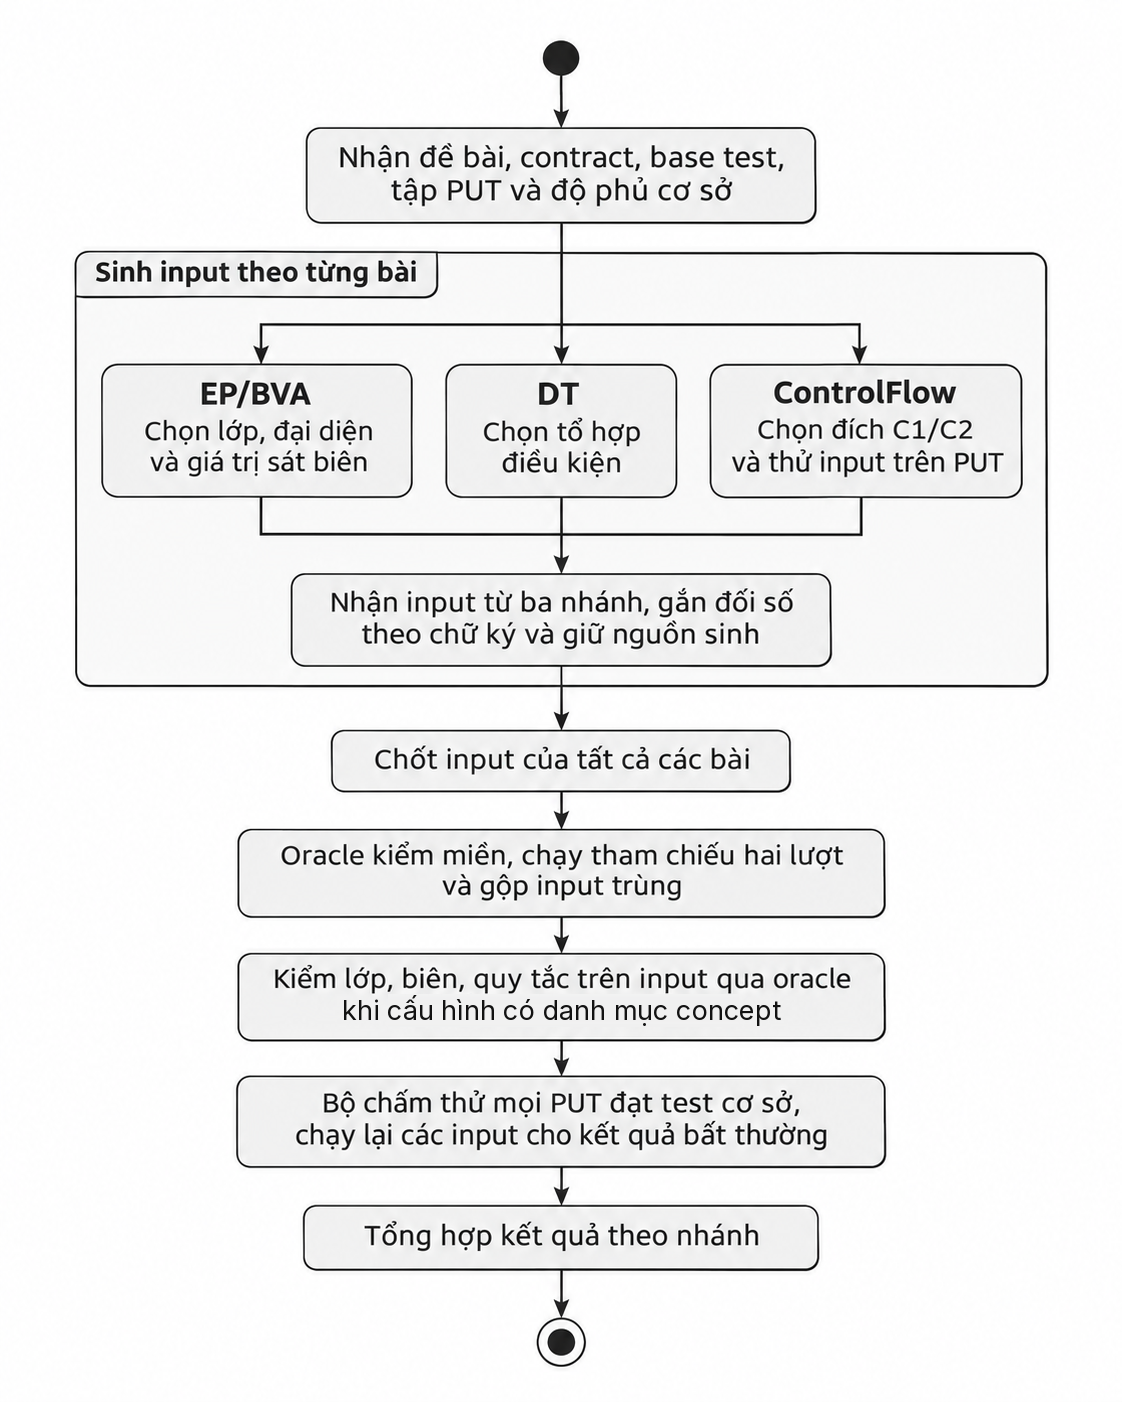
\includegraphics[width=\linewidth,height=.68\textheight,keepaspectratio]{diagrams/hinh2_1-danh-muc-concept.png}
\caption[Pipeline ConceptTesting]{Pipeline ConceptTesting với ba nhánh sinh input độc lập trên dữ liệu của mỗi bài. Đề xuất từ ba nhánh được đưa về bước xử lý chung.}
\label{fig:architecture}
\end{figure}

Hệ thống đọc đề bài và thông tin miền từ benchmark, đồng thời lấy nguồn tham chiếu cho bước oracle. Ngữ cảnh của mỗi bài gồm đặc tả, chữ ký hàm, contract, base test và mã PUT. Trong thực nghiệm HumanEval, pipeline xử lý những bài có đủ mười cài đặt, trong đó ít nhất một cài đặt vượt base test.

Danh mục concept (\textit{concept catalogue}) ghi các lớp tương đương và giá trị biên của EP/BVA, hoặc các điều kiện và quy tắc quyết định của DT. Hệ thống đối chiếu danh mục với các input đã sinh để xác định mục nào đã được thử và mục nào còn thiếu.

EP/BVA và DT dùng chung một ngữ cảnh. Hệ thống lược chú thích và docstring khỏi bản mã PUT gửi đi, rồi tính số token của ngữ cảnh và hướng dẫn để chừa chỗ cho phản hồi. Khi cần, hệ thống giảm số PUT được đưa vào ngữ cảnh. Các cấu hình dùng phản hồi từ danh mục concept giữ nguyên ngữ cảnh đã chọn và báo thiếu chỗ nếu prompt vượt giới hạn. ControlFlow dựng ngữ cảnh riêng từ các PUT có đích chưa phủ.

Các nhánh được chọn sinh input cho từng bài. Hệ thống chốt input của tất cả các bài trước khi chạy oracle. Trên HumanEval, sau hai lượt chạy tham chiếu, hệ thống gộp các input được giữ theo khóa chuẩn hóa và ghi các nhánh đã sinh từng input trước khi chấm PUT. Trong các bảng kết quả, ConceptTesting gồm EP/BVA, DT và ControlFlow. Kết quả chính trên HumanEval dùng biến thể ControlFlow theo nghĩa vụ trình bày ở Mục~\ref{sec:obligation-pipeline}. Naive LLM dùng ngữ cảnh chung để sinh đối số trực tiếp và được báo riêng làm baseline.

\subsection{Khác biệt về ngữ cảnh giữa HumanEval và MBPP}

HumanEval cung cấp prompt theo dạng chữ ký hàm, docstring và entry point rõ ràng. Ngữ cảnh giữ phần mô tả hàm cùng chữ ký, rồi bổ sung contract, base test và mã PUT. MBPP cung cấp mô tả bài toán bằng văn bản cùng các test công khai; bước chuẩn bị bổ sung chữ ký để mô hình biết tên hàm và các tham số. Chỉ giao diện của hàm được dùng ở đây; thân lời giải tham chiếu được dành cho oracle.

Prompt MBPP đặt mô tả, chữ ký và ví dụ thành các phần mà mô hình có thể đọc cùng nhau. EP/BVA, DT và ControlFlow gốc dùng các phần này theo cùng cách như trong cấu hình ablation một lượt trên HumanEval. Prompt chỉ đưa ràng buộc miền mà dữ liệu cho phép xác định. Phần đánh giá MBPP trình bày riêng mức kiểm miền thực tế.

\subsection{Ngữ cảnh và hướng dẫn theo concept}
\label{sec:concept-guidance}

Trong ngữ cảnh đầu vào, đặc tả và contract xác định hành vi cùng miền input của bài, test cơ sở cho mô hình thấy những lời gọi đã có, còn mã PUT có thể gợi ra một cách hiểu sai đặc tả, chẳng hạn một phép so sánh chặt ở cận làm cho giá trị ngay tại cận đáng thử. Từ cùng ngữ cảnh này, Naive LLM sinh input trực tiếp thay vì đi qua bước hướng dẫn theo concept.

Ở lượt đầu, EP/BVA hướng mô hình tìm lớp đầu vào theo hành vi và chọn đại lượng cần thử quanh biên. DT hướng mô hình tìm các tổ hợp điều kiện có thể làm đổi hành động hoặc thứ tự ưu tiên. Giả thuyết về lỗi giúp chọn lớp hoặc quy tắc đáng thử ở cả hai nhánh. Với ControlFlow, hệ thống đối chiếu mã PUT với độ phủ cơ sở để đưa dòng, cạnh chưa phủ và đường gợi ý vào ngữ cảnh. Từ đường gợi ý, mô hình mô tả concept dưới dạng quan hệ giữa các đối số rồi đề xuất cách dựng input đưa PUT tới đích.

Để hệ thống có thể kiểm các đề xuất, mô hình ghi giá trị dưới tên tham số tương ứng. Một mảng JSON dưới tên tham số danh sách biểu diễn một đối số. Tuple và set có thêm thẻ kiểu để khôi phục đúng đối tượng Python. Mô hình có thể gửi ít input hơn giới hạn để tránh lặp lời gọi.

Sau lượt đầu, EP/BVA và DT loại lời gọi trùng nhau hoặc trùng test cơ sở rồi đối chiếu các đối số với danh mục concept. Khi contract có thể kiểm bằng biểu thức, phép đo chỉ dùng input thỏa contract. EP/BVA kiểm input thuộc lớp nào và đã chạm những mốc biên nào. DT tính giá trị các điều kiện trên đối số để xác định quy tắc khả thi nào đã được thử. Nếu còn đủ chỗ trong cửa sổ ngữ cảnh, lượt hai giữ nội dung ban đầu và thêm bản tóm tắt danh mục, các mục chưa phủ hoặc chưa xác định, các lỗi kiểm tra và input đã giữ. Dựa trên phản hồi này, mô hình được hướng dẫn sinh thêm ca cho các mục còn thiếu và rà các tình huống ngoài danh mục ban đầu. Hệ thống tiếp tục dùng danh mục lượt đầu làm mốc đo độ phủ.

Với ControlFlow, hệ thống chạy thử các input trên PUT có đích. Nếu concept có biểu thức, hệ thống tính biểu thức đó trên các bộ đối số gắn với concept. Dấu vết thực thi cho biết input có thực sự đi qua dòng hoặc cạnh cần phủ hay không. Khi cùng một lô còn đích chưa chạm hoặc lỗi đọc phản hồi và còn lượt sửa, hệ thống gửi lại các đích còn thiếu, concept đã đọc và kết quả kiểm concept. Phản hồi kèm tối đa mười hai quan sát, mỗi quan sát ghi lời gọi đã thử, trạng thái kiểm miền, trạng thái thực thi và các đích đã chạm. Mô hình dùng thông tin này để sửa cách dựng input hoặc điều chỉnh quan hệ đã đề xuất. Sau khi chốt input, hệ thống mới lấy đáp án từ bản tham chiếu và chấm PUT.

Bài HumanEval/125 ở phần Mở đầu nhận một chuỗi và dùng ba quy tắc trong Bảng~\ref{tab:word-split-rules}. Nếu chuỗi có khoảng trắng, hàm trả danh sách từ tách theo khoảng trắng. Nếu thiếu khoảng trắng nhưng có dấu phẩy, hàm tách theo dấu phẩy. Khi thiếu cả hai, hàm đếm chữ cái thường có chỉ số lẻ trong bảng chữ cái, với \texttt{a} ở vị trí 0.

PUT 4 tách chuỗi theo khoảng trắng khi xét số phần, nhưng chỉ trả danh sách từ nếu chuỗi chứa dấu cách thường. Với \texttt{a\textbackslash tb}, thao tác tách cho hai từ. Phép kiểm dấu cách thường lại cho kết quả sai, và chuỗi cũng thiếu dấu phẩy, nên PUT chuyển sang nhánh đếm. Nó trả \texttt{1} vì chỉ có \texttt{b} mang chỉ số lẻ trong bảng chữ cái. Tab thuộc nhóm khoảng trắng nên đáp án theo đặc tả là \texttt{['a', 'b']}. Mục~\ref{sec:demo} trình bày cách ControlFlow chọn input để làm lộ sai khác này.

Hình~\ref{fig:ep-bva} minh họa ngữ cảnh lượt đầu mà EP/BVA và DT dùng chung. Trong đó, mã của mười PUT chiếm 1.441 trong 1.764 token nội dung. Với ControlFlow, Hình~\ref{fig:cf-context} cho thấy kết quả chạy thử được đưa vào ngữ cảnh lượt sửa. Số token trên các hình chỉ tính phần nội dung minh họa. Hướng dẫn hệ thống và định dạng hội thoại dùng thêm token.

\begin{figure}[!htbp]
\centering
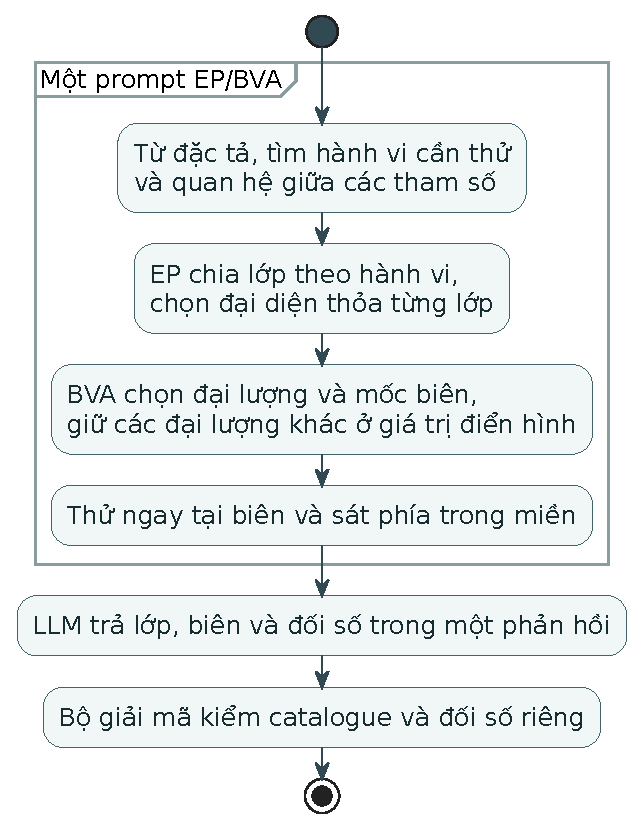
\includegraphics[scale=.70]{diagrams/ep-bva.pdf}
\caption{Các khối ngữ cảnh chung của EP/BVA và DT ở lượt đầu trên HumanEval/125.}
\label{fig:ep-bva}
\end{figure}

\section{EP và BVA trong cơ chế sinh hai lượt}
\label{sec:ep-bva}

\subsection{EP chọn lớp theo hành vi}

Cả ngày 31 tháng 4 lẫn ngày 31 tháng 5 đều truyền được dưới dạng chuỗi. Hàm kiểm tra ngày phải từ chối ngày thứ nhất và chấp nhận ngày thứ hai. Hai ca cần thuộc hai lớp dù từng trường ngày và tháng cùng nằm trong các khoảng số quen thuộc. Vì vậy, phần EP của prompt yêu cầu đọc quan hệ giữa các tham số, gom đầu vào theo quy tắc xử lý rồi chọn đại diện cho mỗi lớp.

Ví dụ về bộ lọc phiên bản đi kèm prompt cho thấy khi nào nên tách một lớp để kiểm một giả thuyết lỗi. Với ngưỡng từ 2.0, thêm bản chính thức 1.9 vào danh sách chỉ có bản thử 2.1a1 vẫn phải giữ 2.1a1. Bản 1.9 không qua ngưỡng, nên sau khi lọc vẫn chưa có bản chính thức phù hợp. Một cài đặt loại bản thử ngay khi thấy 1.9 sẽ cho kết quả khác giữa hai danh sách. Ví dụ lấy từ miền khác để mô hình áp dụng cách suy luận vào bài đang xét. Mô hình có thể lưu giả thuyết về thứ tự lọc cùng mô tả lớp~\cite{packagingVersions}.

\subsection{BVA chọn đại lượng và giữ bối cảnh}

Để thử cận ngày của tháng 4, thay ngày 29 bằng ngày 30 và giữ nguyên tháng, năm, vì đổi cả tháng có thể khiến hai lời gọi kiểm hai quy tắc khác nhau. Phần BVA của prompt yêu cầu mô hình làm tương tự với các lớp đã xác định: trước hết chọn đại lượng cần thử (có thể là giá trị số, độ dài chuỗi, số lần xuất hiện của một phần tử hoặc số chuyển từ chuỗi), cận theo đặc tả và một bộ đối số điển hình. Với cận nguyên hữu hạn, hướng dẫn ưu tiên giá trị tại cận và giá trị kề phía trong lớp, trong khi EP vẫn chọn đại diện ở bên trong lớp; cả hai phần dùng chung ngân sách và mô hình có thể giữ ca khác nếu ca đó phân biệt được một giả thuyết lỗi riêng.

Trường \texttt{covers} lưu liên kết do mô hình khai báo giữa một bộ đối số với lớp hoặc biên được nhắm tới. Khi gộp các input trùng, hệ thống giữ nguồn của liên kết. EP và BVA dùng chung một tập input trong cấu hình này, nên số PUT phát hiện được tính cho cả nhánh.

\subsection{Kiểm tra lớp, biên và vòng bổ sung điểm mù}

Một input được gắn nhãn lớp vẫn cần thỏa điều kiện của lớp đó. Ở lượt đầu, EP/BVA dùng lược đồ JSON bắt buộc để mô hình trả về tối đa 20 input mới cùng danh mục concept (Hình~\ref{fig:ep-bva-dt-flow}). Danh mục ghi bộ đối số danh định dùng chung (\texttt{nominal}), các lớp rời nhau kèm điều kiện kiểm được và các biên rút từ đặc tả. Với đại lượng đếm, danh mục ghi giá trị cần đếm. Các trường mô tả lớp dài được lược bỏ.

Sau lượt đầu và trước khi gọi oracle, hệ thống kiểm miền, mã trùng và thứ tự cận, rồi đối chiếu danh mục concept với các input đã giữ để đo độ phủ. Nếu lớp khai báo tập giá trị, khoảng trên đại lượng xác định được hoặc biểu thức điều kiện, bộ đo tính trực tiếp trên đối số đã gắn tên; với lớp chỉ có mô tả bằng lời, nhãn giữ ở trạng thái chưa xác định. Một phần tử thay đổi trong danh sách có thể giữ nguyên độ dài nhưng làm đổi số lần xuất hiện của giá trị đang xét, nên khi kiểm BVA, bộ đo so cả các đại lượng rút ra từ cùng một tham số với bộ đối số danh định, tính mốc tại các cận hữu hạn, tìm giá trị kề và kiểm mốc trong bối cảnh đã khai báo. Với số thực, bước nhảy lấy từ đặc tả nếu có; nếu không, hệ thống dùng giá trị biểu diễn được liền kề.

Ở lượt hai, nhánh giữ nguyên tiền tố ngữ cảnh của lượt đầu, bổ sung bản tóm tắt chỉ đọc về danh mục concept ở lượt đầu, danh sách các lớp hoặc biên chưa chạm, chưa xác định, lỗi metadata (không lặp lại mục tiêu đã phủ) cùng các input đã giữ. Lượt này chuyển sang JSON tự do (không áp \texttt{json\_schema} cứng) với tối đa 20 input mới khác biệt (tổng trần giữ lại 40 input mỗi task), để mô hình lấp nốt mục tiêu còn thiếu của lượt một và rà soát thêm các điểm mù ngoài khung lớp và biên đã khai báo. Danh mục của lượt đầu vẫn được giữ nguyên làm chuẩn đo phủ chính thức trên toàn bộ tập input hợp lệ từ cả hai lượt.

\begin{figure}[!htbp]
\centering
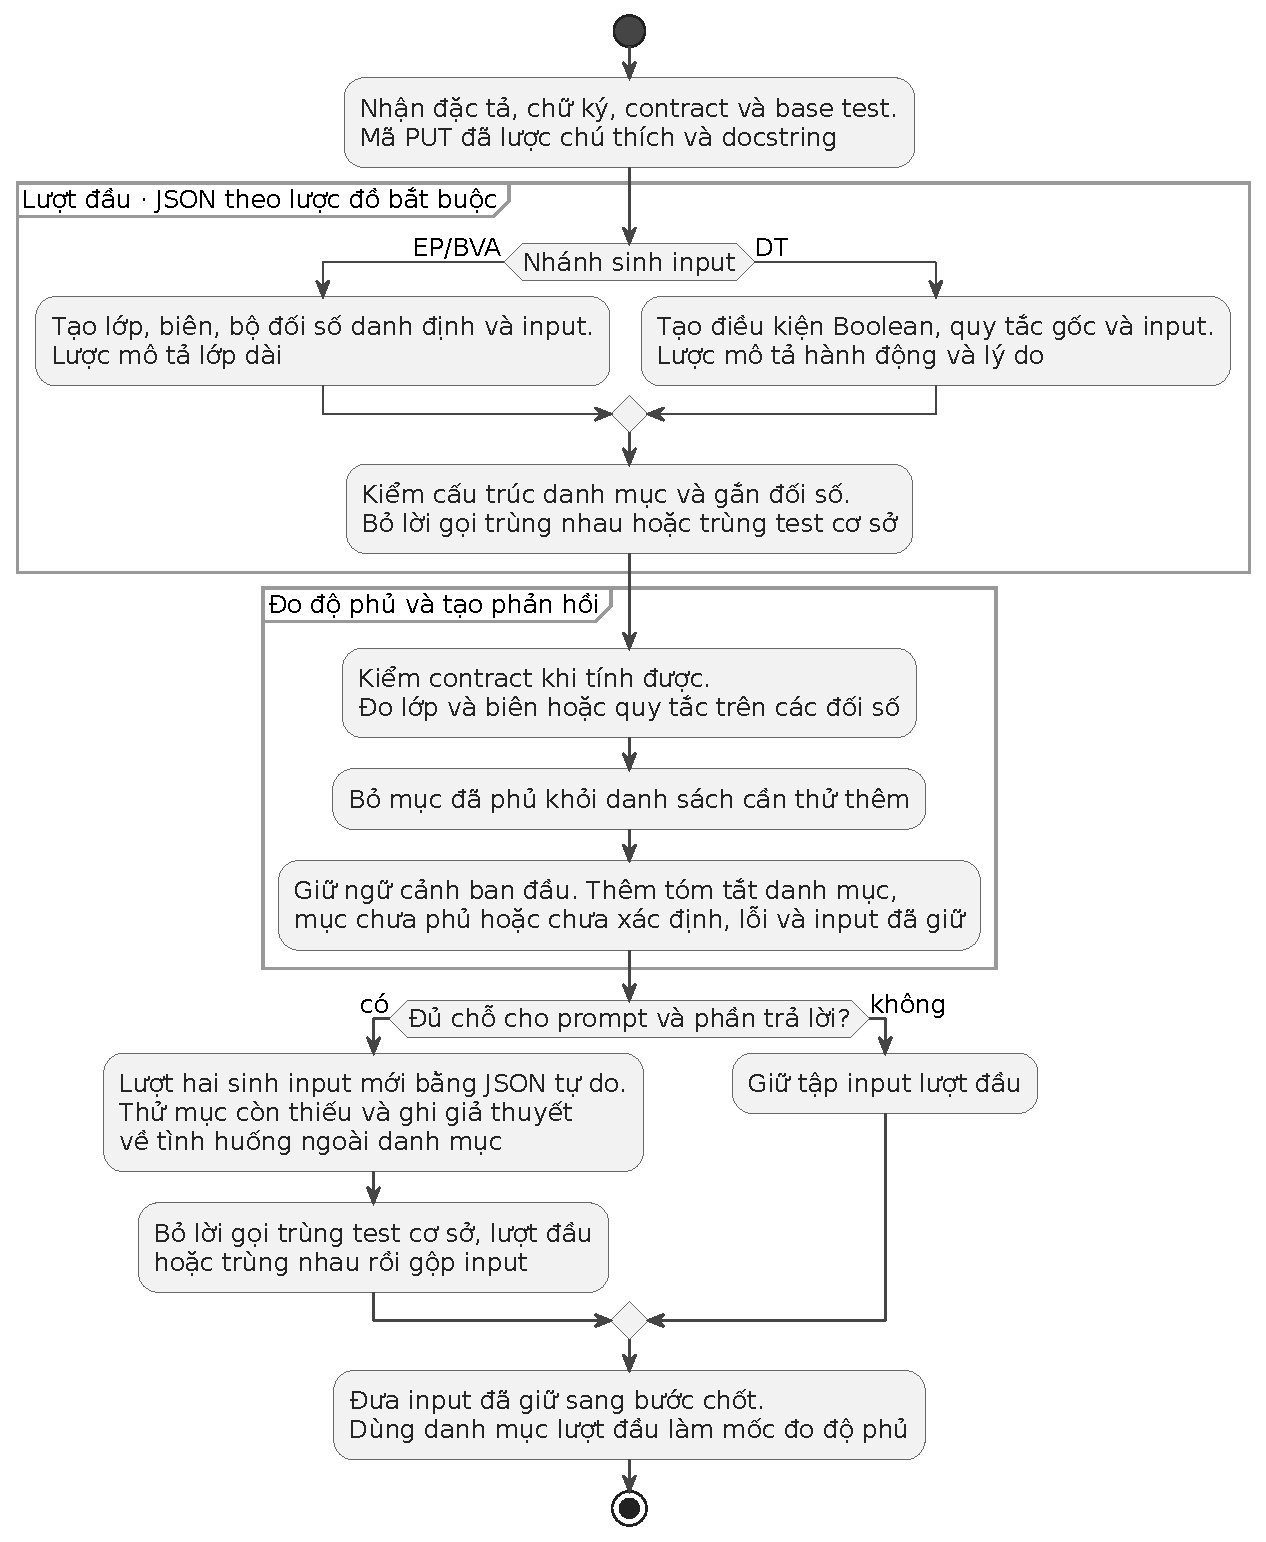
\includegraphics[width=\linewidth,height=.76\textheight,keepaspectratio]{diagrams/ep-bva-dt-flow.pdf}
\caption{Luồng sinh input hai lượt của EP/BVA và DT.}
\label{fig:ep-bva-dt-flow}
\end{figure}

\section{DT chọn đầu vào theo bảng quyết định}
\label{sec:dt}

DT dùng ngữ cảnh chung ở Hình~\ref{fig:ep-bva} và đi theo nhánh DT ở Hình~\ref{fig:ep-bva-dt-flow}. Hướng dẫn sinh yêu cầu mô hình lập quy tắc từ các điều kiện có thể xuất hiện đồng thời. Một ca chỉ có khoảng trắng và một ca chỉ có dấu phẩy đều có thể đạt dù cài đặt ưu tiên sai khi gặp cả hai. Tổ hợp có cả hai dấu phân cách cần một ca riêng để kiểm thứ tự ưu tiên.

Với mỗi tổ hợp, mô hình ghi nhận tính khả thi, mâu thuẫn với đặc tả hay tình trạng thiếu thông tin; việc ghi rõ tổ hợp mâu thuẫn giúp tránh sinh lời gọi không dùng được. Khi rút gọn bảng, chỉ nên gộp hai quy tắc nếu hành động và thứ tự giữ nguyên dưới cả hai giá trị của điều kiện định bỏ, còn khi nghi cài đặt ưu tiên sai, cần giữ hai input chỉ khác nhau ở điều kiện quyết định để phân biệt hai hành vi.

Trong ví dụ HTTP của prompt, thẻ phiên bản trong \texttt{If-None-Match} khớp tài nguyên ở cả hai lời gọi nhưng GET nhận mã 304 còn PUT nhận mã 412~\cite{fielding2022http}; vì đổi phương thức làm đổi hành động, hai trường hợp cần được giữ riêng. Ví dụ cũng có trường hợp sự xuất hiện của một điều kiện khiến điều kiện về thời gian mất tác dụng. Khi áp dụng vào một task khác, mô hình phải lấy điều kiện và hành động từ đặc tả của task đó.

Phản hồi lượt đầu của DT tuân theo lược đồ JSON bắt buộc gọn, với tối đa 20 input mới khác biệt. Mô hình tách từ một đến bốn điều kiện Boolean kèm biểu thức trên tên tham số và đánh dấu từng hàng là khả thi, mâu thuẫn hoặc chưa xác định. Một input khớp với một hàng khi mỗi biểu thức trả đúng giá trị \texttt{True} hoặc \texttt{False} mà hàng đó yêu cầu. Một giá trị khác với yêu cầu đủ để bác liên kết giữa input và hàng đó. Nếu còn biểu thức chưa đánh giá được và các giá trị đã tính đều khớp, kết quả đối chiếu vẫn chưa xác định. Trường \texttt{covers} lưu các nhãn do mô hình khai báo. Mẫu số độ phủ là số hàng gốc được đánh dấu khả thi.

Sau lượt đầu và trước bước oracle, hệ thống kiểm miền tin cậy, đo phủ quan sát các quy tắc khả thi và trích riêng danh sách quy tắc chưa chạm, chưa xác định cùng các điều kiện gặp lỗi thực thi (không lặp lại phần đã phủ). Khi contract kiểm được, phép đo dùng các input đã qua kiểm miền; ngược lại, kết quả đo chỉ mang tính tạm thời.

Ở lượt hai, DT giữ nguyên tiền tố ngữ cảnh của lượt đầu và bổ sung bản tóm tắt chỉ đọc về bảng điều kiện, các quy tắc còn thiếu hoặc lỗi thực thi cùng tập input đã giữ. Lượt này cũng dùng JSON tự do (không ép \texttt{json\_schema} cứng và không yêu cầu chép lại bảng quy tắc) với tối đa 20 input mới khác biệt (tổng trần 40 input mỗi task) để bổ sung các tổ hợp điều kiện còn thiếu, đồng thời kiểm các tương tác biên và giả thuyết lỗi nằm ngoài bảng điều kiện lượt một. Bảng quy tắc lượt một giữ nguyên làm chuẩn đo phủ cho toàn bộ tập input hợp lệ sau khi gộp và loại trùng từ cả hai lượt.

\section{ControlFlow chọn đích trong mã nguồn}
\label{sec:control-flow}

\subsection{Tìm dòng và cạnh còn thiếu}

ControlFlow xét toàn bộ PUT đã vượt base test. Khi đã có số đo cơ sở, nhánh dùng tập dòng và cạnh đã quan sát. Nếu thiếu số đo, nhánh thử lại tối đa 300 lời gọi cơ sở đã ghi cho mỗi PUT. Trạng thái độ phủ vẫn là chưa xác định nếu phép đo chưa đủ. Nếu cấu hình cấp thêm một tập input, nhánh chạy các input đó để cập nhật mốc độ phủ trước khi tìm đích còn thiếu.

\textit{coverage.py} đọc mã nguồn để lấy các dòng có thể thực thi, cạnh chuyển dòng và số lối ra. ControlFlow nhóm các cạnh theo dòng xuất phát rồi duyệt theo chiều rộng từ lệnh đầu tiên trong thân hàm sau chuỗi mô tả. Với mỗi dòng mới trong phạm vi hàm, nhánh giữ đường đầu tiên tìm được. Dòng thực thi có đường tới và chưa được test cơ sở chạy qua trở thành đích C1. Từ một dòng có nhiều lối ra, cạnh nào chưa được đi qua là đích C2. Mỗi đích đi kèm PUT, vị trí, đoạn mã và đường gợi ý. Đường tìm trên đồ thị vẫn có thể chứa hai điều kiện mâu thuẫn khi chuyển thành giá trị cụ thể.

\subsection{Prompt khám phá, chạy thử và sửa đề xuất}

ControlFlow xếp đích theo thứ tự phân tích. Để tạo một lô, nhánh lấy tối đa sáu đích đầu danh sách sao cho đích, đường gợi ý, mã PUT liên quan và tối đa mười hai lời gọi cơ sở mỗi PUT cùng vừa cửa sổ ngữ cảnh. Các đích còn lại chuyển sang lô kế tiếp. Một đích chỉ bị bỏ khi gửi riêng vẫn vượt giới hạn. Mỗi lô nhận một lượt sinh đầu. Nếu còn lượt sửa và lô cuối vẫn có đích chưa chạm hoặc lỗi, phản hồi được gửi lại cho lô đó.

Chẳng hạn, ở HumanEval/125, lượt đầu chứa mã PUT 4, các lời gọi cơ sở và đích C2 \(8\rightarrow12\). Phần phản hồi ở lượt sửa chiếm 1.044 trong 1.741 token nội dung vì có thêm concept, kết quả kiểm và các lời gọi đã thử (Hình~\ref{fig:cf-context}).

\begin{figure}[!htbp]
\centering
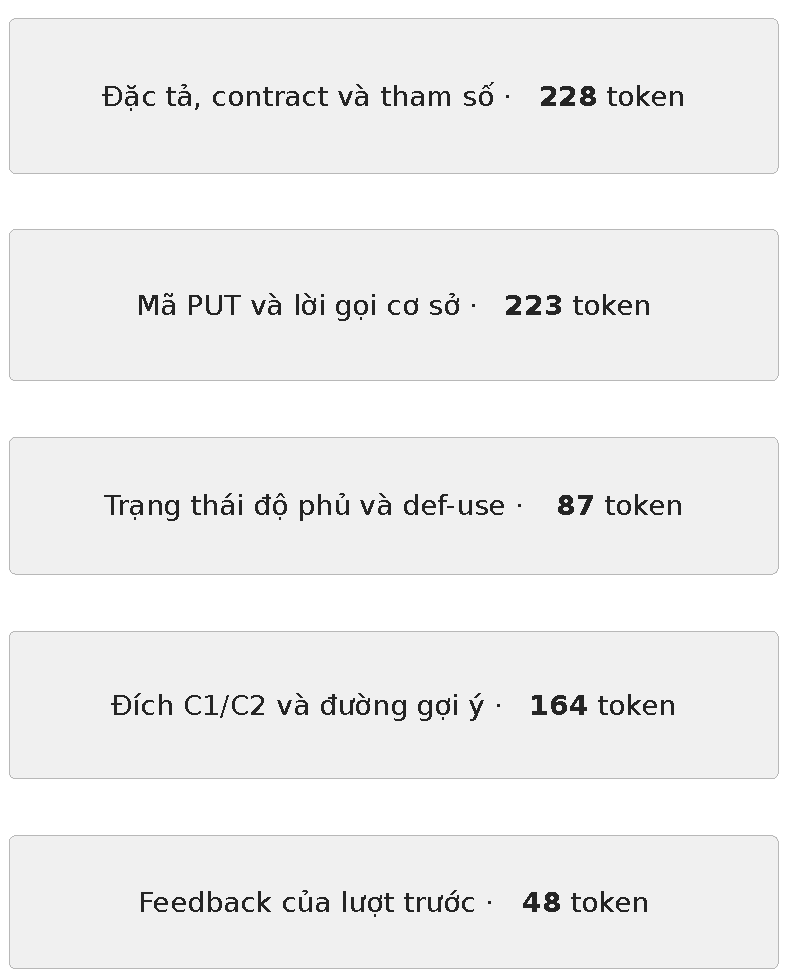
\includegraphics[scale=.70]{diagrams/control-flow-context.pdf}
\caption{Các khối ngữ cảnh của ControlFlow ở lượt sửa trên HumanEval/125.}
\label{fig:cf-context}
\end{figure}

Một bộ đối số có thể thỏa phép so sánh cuối mà vẫn bị chặn bởi điều kiện trước đó. Ở lượt đầu, mô hình dùng mã đích và số dòng để tìm vị trí, lần qua các điều kiện trước đó rồi mô tả concept bằng một quan hệ trên input và cách dựng đối số thỏa quan hệ ấy. Phản hồi có thể thêm biểu thức trên tham số và miền lấy mẫu. Khi quan hệ chỉ diễn đạt được bằng lời, trường biểu thức có thể để trống. Một biểu thức hằng đúng không giới hạn được input.

\begin{figure}[!htbp]
\centering
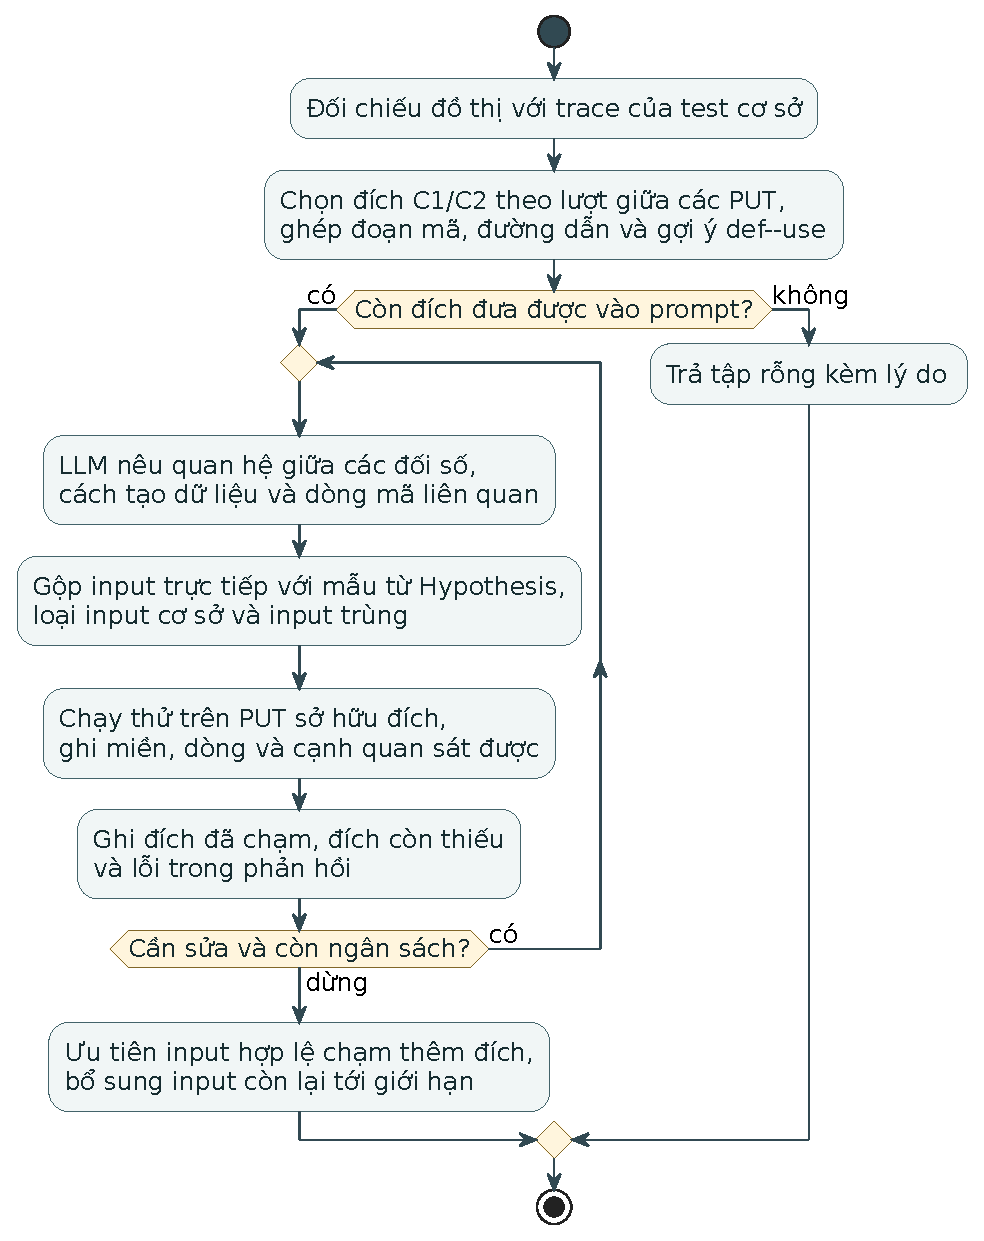
\includegraphics[width=\linewidth,height=.70\textheight,keepaspectratio]{diagrams/control-flow.pdf}
\caption{Vòng phản hồi ControlFlow. Thông tin về miền, kết quả kiểm concept và đường chạy giúp mô hình sửa đề xuất.}
\label{fig:cf-mechanism}
\end{figure}

Bộ giải mã đối chiếu mã đích, dòng và chữ ký trước khi nhận các trường của concept, đồng thời yêu cầu biểu thức dùng cú pháp được phép, phụ thuộc vào tham số và miền lấy mẫu gắn đúng tên tham số của hàm. Hypothesis có thể lấy thêm mẫu từ mô tả đó, chẳng hạn danh sách có giới hạn độ dài và kiểu phần tử. Một input trực tiếp vẫn được xét dù mô tả concept đi kèm có lỗi; nếu cả hai nguồn đưa cùng bộ đối số, hệ thống thử một lần và lưu cả hai nguồn. Sau khi bỏ lời gọi trùng với test cơ sở, lượt chạy ưu tiên input trực tiếp trong phần ngân sách còn lại.

Sau khi chạy thử input trên các PUT sở hữu đích, nhánh so dòng và cạnh đã đi qua với vị trí C1/C2. Ngân sách mặc định là 64 lượt quan sát input--PUT cho đề xuất của mô hình, và nhánh có thể tăng ngân sách để dự trữ một lượt quan sát cho mỗi PUT ở mỗi lô mới, còn Hypothesis có tối đa 40 lượt lấy mẫu dùng chung trong một bài. Lượt sửa nhận các đích còn thiếu, lỗi giải mã, kết quả kiểm concept và tối đa mười hai quan sát gồm đối số, tình trạng miền, trạng thái chạy và các đích đã chạm (Hình~\ref{fig:cf-mechanism}).

Dựa trên các dòng và cạnh quan sát được khi chạy PUT, ControlFlow ưu tiên input hợp lệ phủ thêm đích rồi dùng chỗ còn lại cho các input hợp lệ khác. Số input tối đa là mức lớn hơn giữa ngân sách đã cấu hình và số đích đã xếp lô cộng 10.

\section{Kết hợp nghĩa vụ theo đặc tả với đích cấu trúc}
\label{sec:obligation-pipeline}

Một dòng đã được phủ vẫn có thể thực hiện sai một yêu cầu của đề bài. Chẳng hạn, test có thể đã đi qua phép cộng nhưng chưa thử hai phần tử bằng nhau trong bài yêu cầu tính mọi lần xuất hiện. Ở cấu hình kết hợp nghĩa vụ theo đặc tả dùng cho kết quả chính trên HumanEval, ControlFlow dùng đặc tả và mã PUT để mô tả điều kiện kích hoạt tình huống đó. Nhánh đồng thời dùng đích C1/C2 để tìm thêm đường chạy mà test cơ sở chưa đi qua.

\begin{figure}[!htbp]
\centering
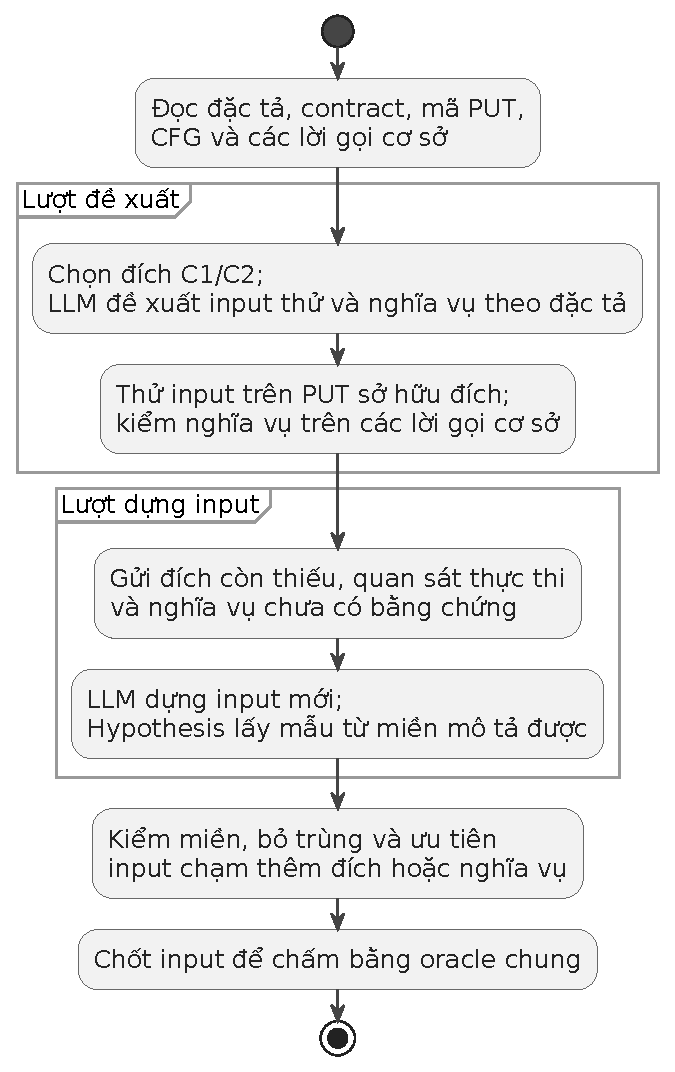
\includegraphics[width=.94\linewidth,height=.66\textheight,keepaspectratio]{diagrams/obligation.pdf}
\caption{Hai lượt sinh ở cấu hình kết hợp nghĩa vụ theo đặc tả và đích C1/C2.}
\label{fig:obligation-pipeline}
\end{figure}

Ở lượt đề xuất, mô hình dùng đặc tả, contract, tên tham số, mã PUT có số dòng, CFG và các lời gọi cơ sở. Nhánh chọn tối đa sáu đích luân phiên giữa các PUT được đưa vào ngữ cảnh. Mô hình đề xuất tối đa sáu nghĩa vụ. Với mỗi nghĩa vụ, nó trích một yêu cầu của đề, gắn vào dòng thực thi của một PUT rồi nêu tình huống, cách dựng input và một trường hợp mà thao tác đó là đúng. Ví dụ đối chiếu giúp phân biệt hai yêu cầu như đếm mọi lần xuất hiện và đếm các giá trị khác nhau. Khi có đích C1/C2, phản hồi đặt input cụ thể ở đầu để bộ đọc còn có thể giữ các bản ghi đối số hoàn chỉnh nếu phần mô tả phía sau bị lỗi.

Đối với nghĩa vụ có biểu thức trên đối số, hệ thống kiểm hai điều kiện trên các lời gọi cơ sở: đối số phải thỏa biểu thức và dấu chạy phải tới dòng đã gắn; khi thiếu biểu thức hoặc dấu chạy, kết quả là chưa xác định. Với mỗi đích C1/C2, hệ thống có thể thử một input mới từ lượt đầu trên PUT sở hữu đích rồi chuyển trạng thái đích sang lượt dựng input: nếu đã chạy xong và trượt đích, phản hồi chỉ ra cạnh đầu tiên trong đường gợi ý chưa quan sát được cùng các lối ra đã thấy để mô hình giữ các điều kiện trước và đổi đối số tại chỗ rẽ cần thử.

Nếu phản hồi đầu chưa đọc được, hệ thống có thể yêu cầu tạo lại một lần. Lượt dựng input ưu tiên giữ mã của PUT sở hữu đích hoặc nghĩa vụ và nhận phần mô tả đã rút gọn để còn chỗ cho các bộ đối số. Mô hình thử đích còn thiếu trước, sau đó dùng ngân sách còn lại cho ca đối chiếu theo đặc tả. Hệ thống kiểm miền, bỏ trùng với lời gọi cơ sở và thử các input trên PUT liên quan trong tối đa 64 lượt quan sát, tính cả các lượt thử trước đó. Nó ưu tiên input chạm thêm đích hoặc nghĩa vụ. Giới hạn hai mươi input áp dụng cho phần mô hình sinh. Mẫu Hypothesis từ các miền có thể diễn giải được dùng ngân sách lấy mẫu riêng và vẫn chịu giới hạn quan sát chung. Các input cuối đi qua cùng quy trình oracle. Trong lần chạy chính trên HumanEval, prompt còn yêu cầu xét độ sâu đệ quy, mức tăng chi phí theo kích thước đầu vào, độ chính xác số thực và giả định về chuỗi hoặc bảng mã. Khi các lời gọi cơ sở đã chạm toàn bộ nghĩa vụ được chọn, nhánh vẫn giữ các nghĩa vụ đó để dựng thêm input đối chiếu.

\section{Chốt dữ liệu, tạo oracle và xác nhận sai khác}
\label{sec:evaluation-pipeline}

\begin{figure}[!htbp]
\centering
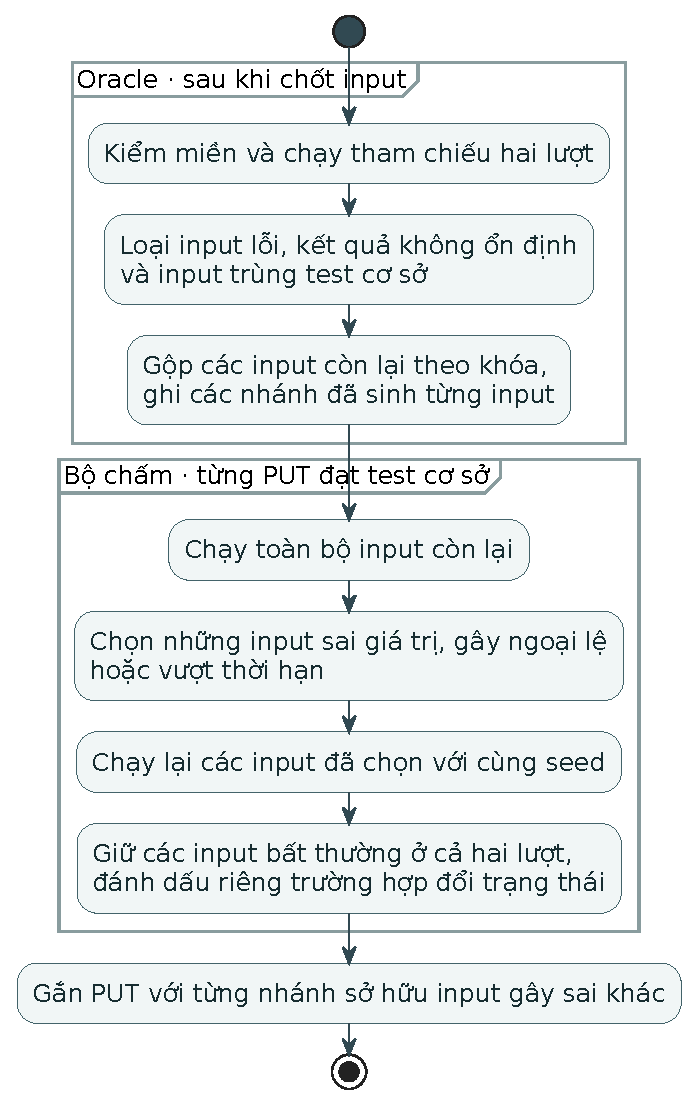
\includegraphics[width=.95\linewidth,height=.63\textheight,keepaspectratio]{diagrams/evaluation.pdf}
\caption{Hai lượt tham chiếu xác định đáp án, còn lượt chạy lại PUT xác nhận kết quả bất thường.}
\label{fig:task-flow}
\end{figure}

Bộ giải mã thử đọc JSON trước. Khi cấu trúc phản hồi cho phép, nó có thể đọc literal Python dưới dạng dữ liệu. Hệ thống lấy chữ ký hàm từ cây cú pháp, gắn đối số theo tên và điền giá trị mặc định. Bước này cũng kiểm tham số thừa hoặc thiếu, độ lồng của dữ liệu và số thực hữu hạn. Hệ thống kiểm riêng trường \texttt{catalogue} chứa danh mục concept, nên một bộ đối số vẫn có thể được đem chấm khi trường mô tả quy tắc bị lỗi.

Để tạo khóa trên HumanEval, hệ thống gắn mỗi đối số vào tham số theo chữ ký hàm rồi điền giá trị mặc định. Quy tắc này áp dụng cho cả lời gọi base test và input đưa vào oracle. Với chữ ký minh họa \texttt{f(x, step=1)}, lời gọi \texttt{f(2)} và \texttt{f(step=1, x=2)} cùng gán \texttt{x=2} và \texttt{step=1}, nên có cùng khóa.

Mỗi giá trị đi vào khóa cùng tên kiểu dữ liệu. Vì vậy, \texttt{True}, \texttt{1} và \texttt{1.0} có ba biểu diễn riêng. Với dữ liệu lồng nhau, hệ thống áp dụng quy tắc này cho từng phần tử, giữ thứ tự của list và tuple, rồi sắp các mục của dict và set theo biểu diễn đã chuẩn hóa. Chuỗi định danh vì thế ổn định cả khi thứ tự duyệt set hoặc thứ tự chèn vào dict thay đổi. Nếu đặc tả có xét thứ tự chèn vào dict, hai lời gọi chung khóa vẫn có thể cần kiểm riêng.

Trước khi chạy thử, ControlFlow lọc đề xuất bằng khóa gồm tên tham số, kiểu và biểu diễn literal của giá trị đã gắn. Ở bước này, hai dict khác thứ tự chèn có thể được giữ để thử riêng. Bước gộp cuối dùng khóa đã chuẩn hóa tại oracle.

Trên MBPP, hệ thống kiểm chữ ký rồi ghi bộ đối số có tên thành JSON với khóa của mỗi đối tượng được sắp xếp. Chuỗi JSON được mã hóa bằng UTF-8 và băm SHA-256. Đổi thứ tự các trường vẫn cho cùng chuỗi để băm. Việc bỏ trống một đối số mặc định và ghi tường minh giá trị đó tạo hai biểu diễn JSON khác nhau trong phép gộp MBPP.

Sau khi chốt input, hệ thống chuyển sang bước lấy đáp án bằng oracle (Hình~\ref{fig:task-flow}). Trên HumanEval, hệ thống kiểm ràng buộc của task rồi chạy bản tham chiếu HumanEval+ hai lần. Một input được giữ nếu cả hai lượt cho cùng khóa đối số, cùng đầu ra và lời gọi chưa xuất hiện trong test cơ sở. Các bản trùng được gộp theo khóa, kèm danh sách nhánh đã sinh input. Nếu có danh mục concept, hệ thống dùng các input còn lại để kiểm lớp, biên và quy tắc trước khi chấm PUT. Trên MBPP, hệ thống cũng chốt đối số trước khi chạy tham chiếu hai lần. Mục~\ref{sec:mbpp-results} ghi giới hạn của phép chấm về kiểm miền và lọc input trùng base test.

Bộ chấm chạy tập input hợp lệ trên mọi PUT vượt base test của bài theo quy tắc so sánh của task, gồm cả sai số cho phép với số thực. Nếu lượt đầu sai giá trị, sinh ngoại lệ hoặc quá giờ, bộ chấm chạy lại chính input đó với cùng seed. Hai lượt bất thường xác nhận một phát hiện. Hai trạng thái khác nhau được ghi nhận là thiếu ổn định. Một nhánh được tính là phát hiện PUT khi có ít nhất một input của nhánh đạt điều kiện xác nhận.
